\documentclass[a4paper,11pt]{article}
\usepackage{polski}
\usepackage[a4paper, left=2cm, right=2cm]{geometry}
\usepackage{xcolor}
\definecolor{grey}{rgb}{0.9,0.9,0.9}
\usepackage[utf8]{inputenc}
\usepackage[T1]{fontenc}
\usepackage[sfdefault,light]{FiraSans}
\usepackage{graphicx}
\usepackage{colortbl}
\usepackage{enumerate}
\usepackage{mathtools}

\renewcommand{\contentsname}{Spis treści}
\usepackage{hyperref}
\hypersetup{
	colorlinks,
	citecolor=black,
	filecolor=black,
	linkcolor=black,
	urlcolor=black
}


\begin{document}
	\begin{titlepage} 
		\begin{center}
			
\includegraphics[scale=0.4]{agh.jpg}
		\end{center}

	
	\begin{center}
		\fontsize{32pt}{80pt}\selectfont
		\vspace{0.7cm}
		Guess X \\ 
		\fontsize{18pt}{30pt}\selectfont
		 Aplikacja Google Home
		\vspace{0.7cm}
	\end{center}

	
		\vfill
		\parbox[t]{0.93\textwidth}{
			\raggedleft
			\large
			{\Large Bartłomiej Pluta}\\[4pt]
			{\Large Aneta Pociecha}\\[4pt]
			{\Large Marek Ochocki}\\[4pt]
			{\Large Magdalena Tragarz}\\[4pt]
		}	
	\end{titlepage}
	
	%---------------------------------------------------------
	
	\newpage
	
	
	\section{Opis systemu}
	
	System pozwala użytkownikowi na uzyskanie określonej informacji poprzez rozmowę z aplikacją. System umożliwia również cykliczne wysyłanie wiadomości na urządzenia obsługujące aplikację Google Assistant.
	
	Użytkownik uruchamia aplikację słowami "Talk to Guess X", składa zapytanie o aktualną wartość x oraz kończy rozmowę poleceniem "bye". Użytkownik może wyrazić zgodę na otrzymywanie powiadomień oraz zrezygnować z subskrypcji.
	
	\paragraph{}
	Technologie:
	\begin{itemize}
		\item firebase functions
		\item firebase realtime database
		\item actions on google
		\item dialogflow
		\item googleapis
		\item nodejs 
		\item typescript
		\item cron job
	\end{itemize}

	Wykorzystane wzorce projektowe:
	\begin{itemize}
		\item fasade
		\item builder
		\item strategy
		\item row data gateway
	\end{itemize}


	\section{Projekt systemu}
	 
    	\begin{figure}[!h]
    		\begin{center}
    			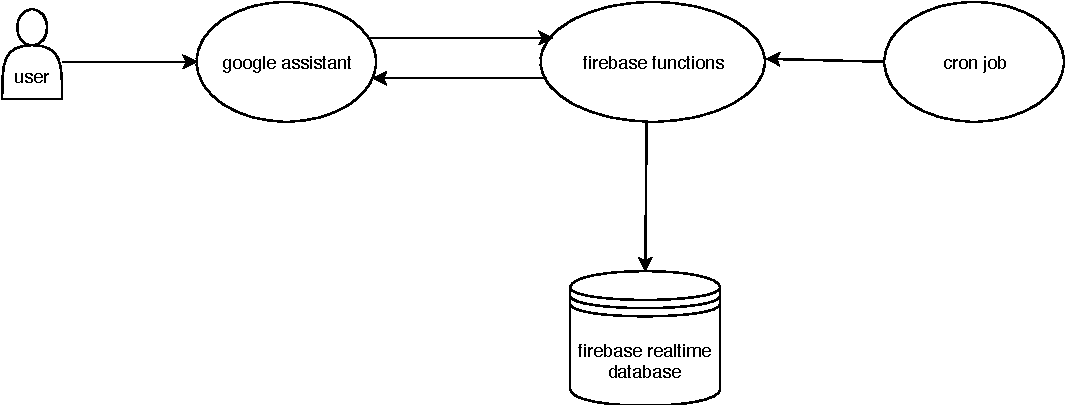
\includegraphics[width=14cm]{guess-x-flow.pdf}
    		\end{center}
    		\caption[Caption for LOF]{Flow}
    		\label{flow}
    	\end{figure}
    
         \begin{figure}[!h]
	    	\begin{center}
	    		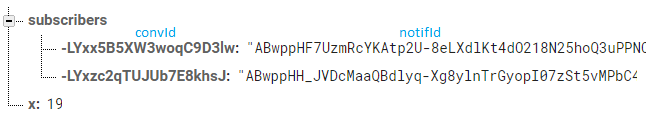
\includegraphics[width=16cm]{db.PNG}
	    	\end{center}
	    	\caption[Caption for LOF]{Struktura bazy danych}
	    	\label{db}
	    \end{figure}
    

        \begin{figure}[!h]
    		\begin{center}
    			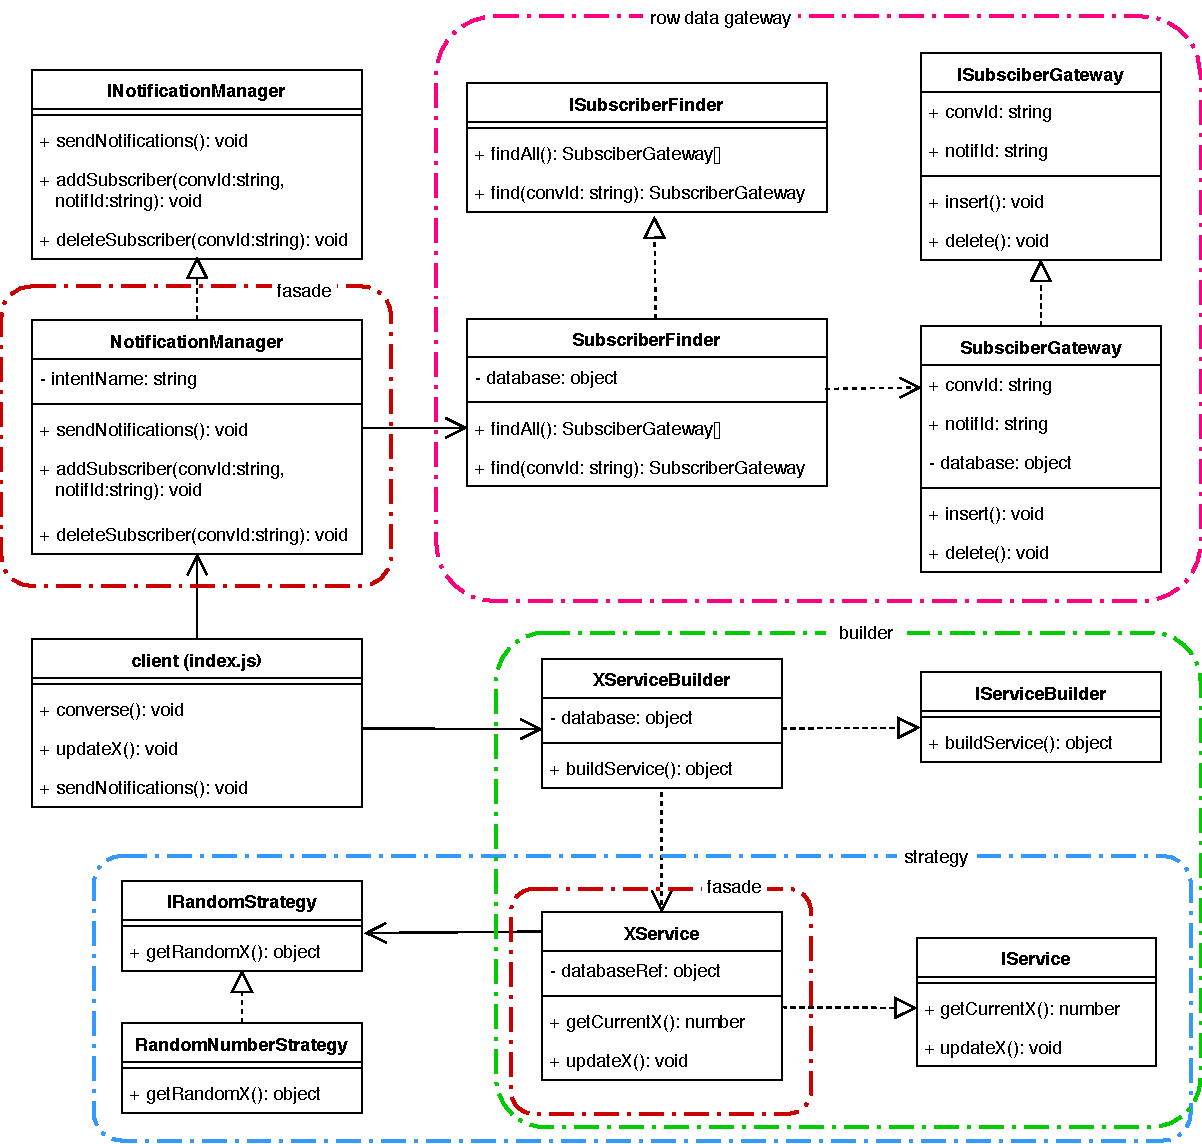
\includegraphics[width=16cm]{guess-x-classes.pdf}
    		\end{center}
    		\caption[Caption for LOF]{Diagram klas serwera}
    		\label{classes}
    	\end{figure}
    
        \begin{figure}[!h]
	    	\begin{center}
	    		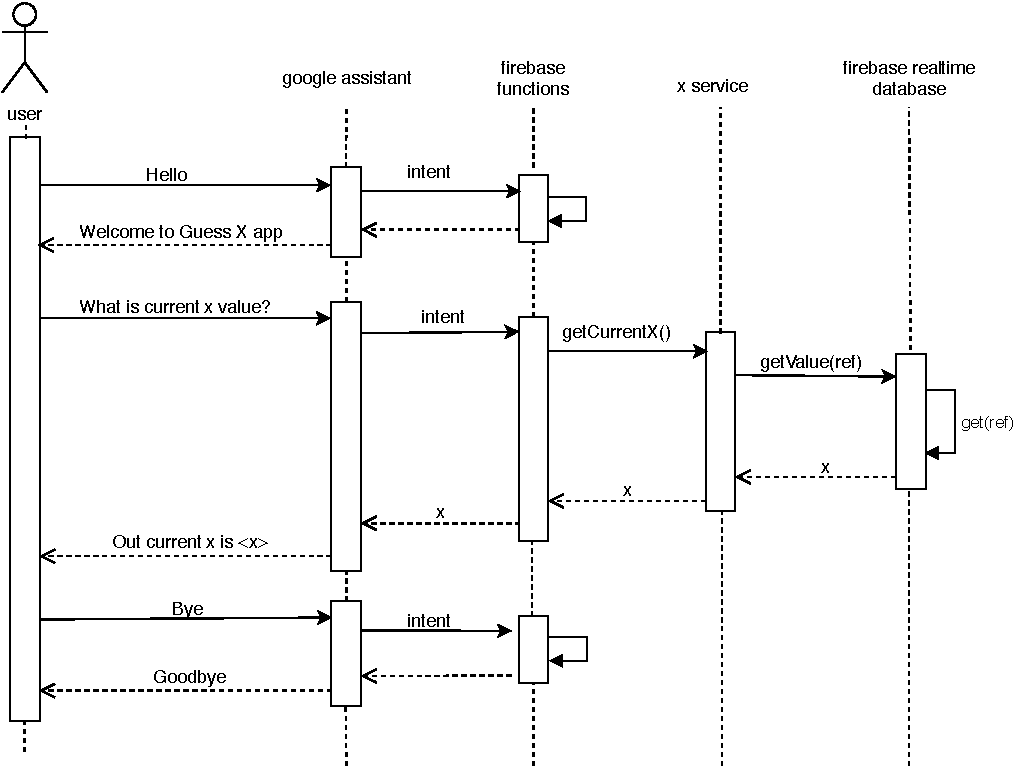
\includegraphics[width=16cm]{guess-x-get-x.pdf}
	    	\end{center}
	    	\caption[Caption for LOF]{Diagram sekwencji - odczytanie wartości x}
	    	\label{getX}
	    \end{figure}
	    
    \begin{figure}[!h]
    	\begin{center}
    		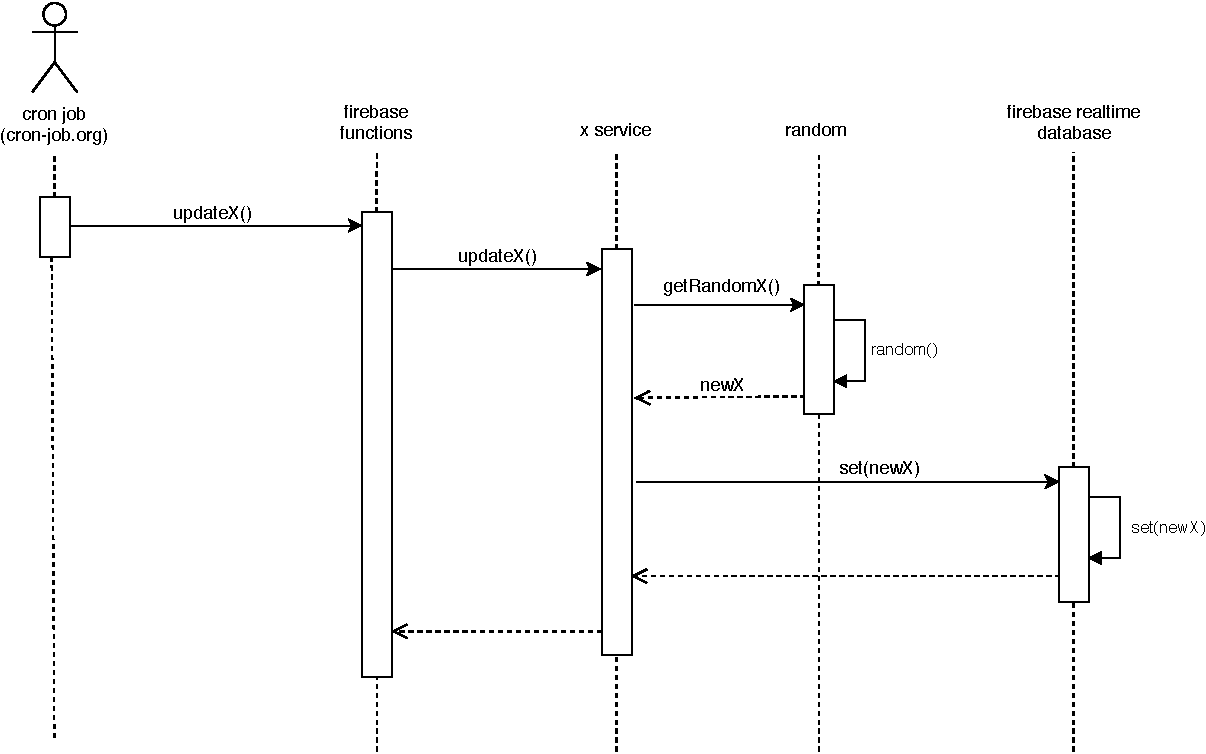
\includegraphics[width=16cm]{guess-x-update-x.pdf}
    	\end{center}
    	\caption[Caption for LOF]{Diagram sekwencji - aktualizacja wartości x}
    	\label{update}
    \end{figure}
    
     \begin{figure}[!h]
    	\begin{center}
    		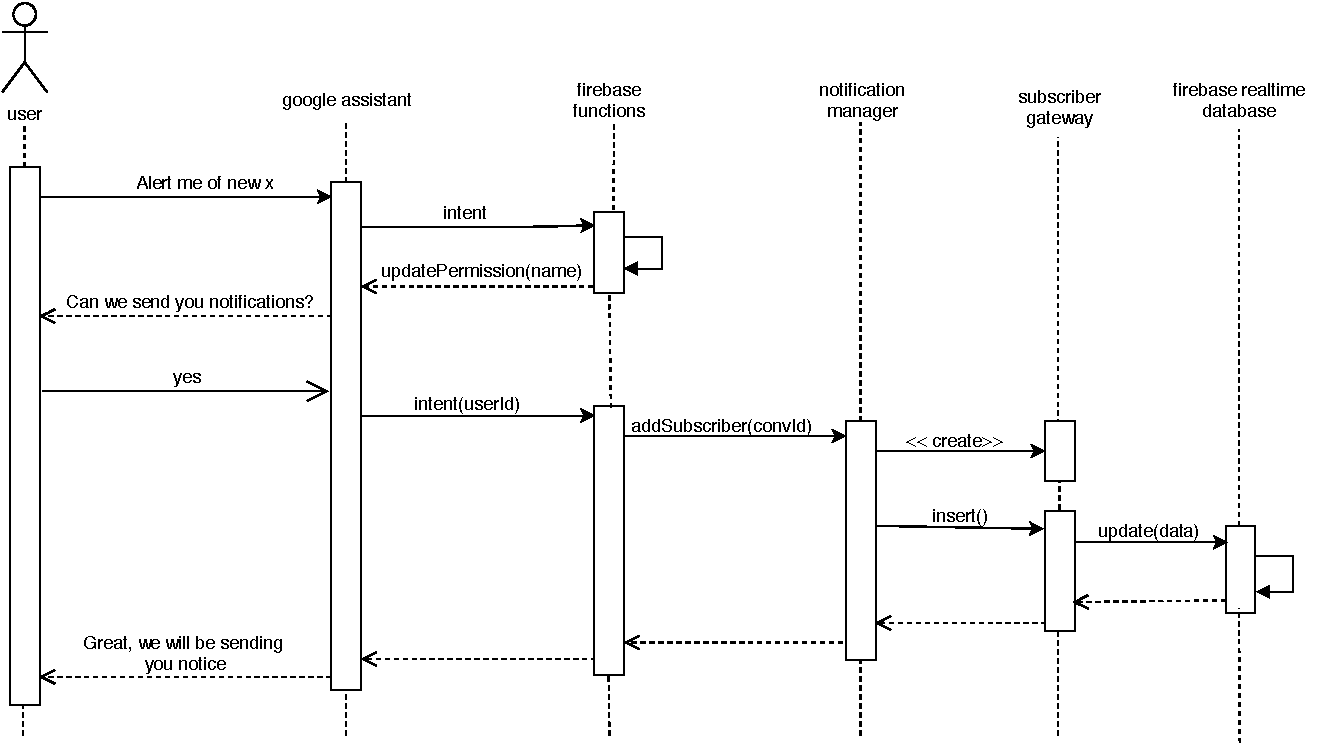
\includegraphics[width=16cm]{guess-x-permission.pdf}
    	\end{center}
    	\caption[Caption for LOF]{Diagram sekwencji - zgoda użytkownika na wysyłanie powiadomień}
    	\label{permission}
    \end{figure}

     \begin{figure}[!h]
		\begin{center}
			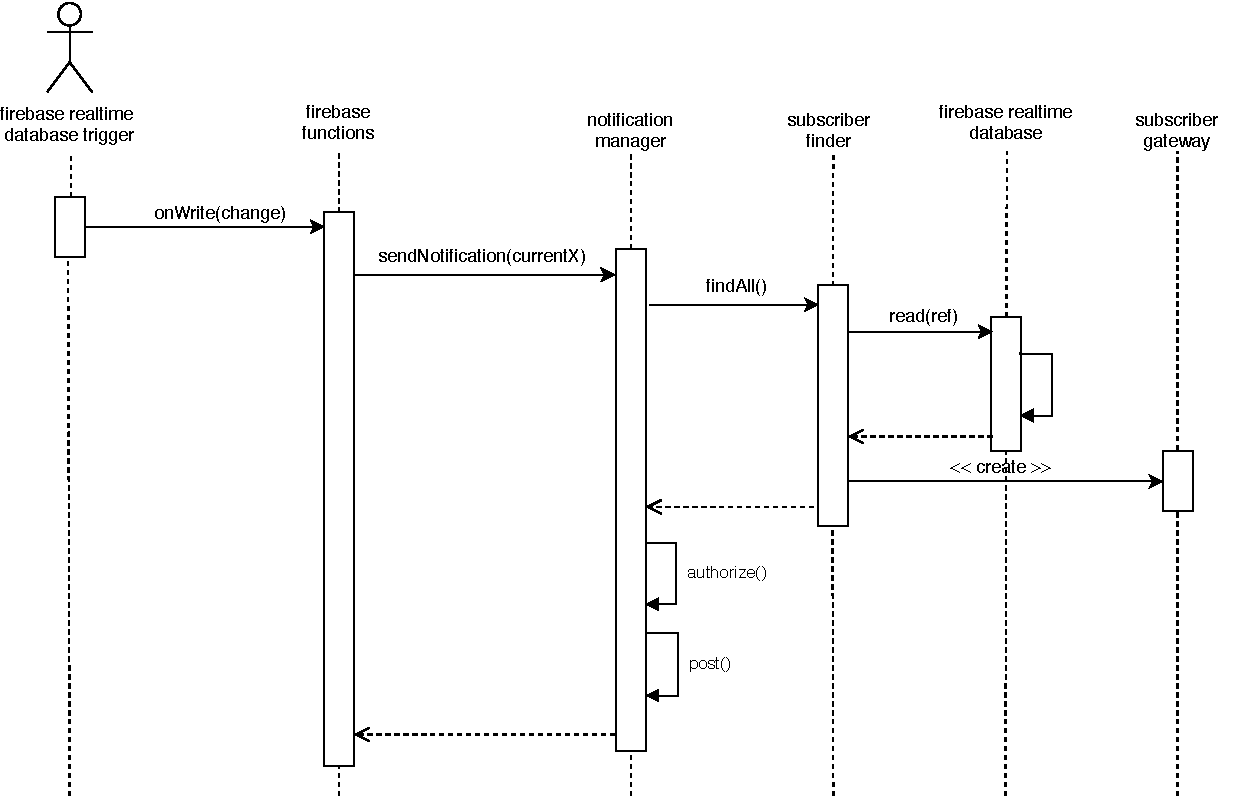
\includegraphics[width=16cm]{guess-x-send-notifications.pdf}
		\end{center}
		\caption[Caption for LOF]{Diagram sekwencji - wysłanie powiadomienia}
		\label{send-notifications}
	\end{figure}




\end{document}